\documentclass[a4paper]{article}

\usepackage[english]{babel}

\usepackage[a4paper,top=2cm,bottom=2cm,left=3cm,right=3cm,marginparwidth=1.75cm]{geometry}

\usepackage[%
  titleformat=italic,% Titles in italic 
  titleformat=commasep,% A comma between athors and title 
  titleformat=all,% Always show a title (or a short title)
  commabeforerest,% A comma after title 
  ibidem=strict,% 
  citefull=first,% The first citing in full form 
  oxford,% The oxford style
  super,% Footnotes 
  dotafter=true,% 
  see,% An extra optional argument as a prenote 
  idem
]{jurabib}

\usepackage[colorlinks=true, urlcolor=blue, linkcolor=black, citecolor=black]{hyperref}
\urlstyle{same}

\usepackage{amsmath}
\usepackage{graphicx}
\usepackage{bbold}

\title{Elliptic curves in modern cryptography}
\author{Andrei Lupsa}

\begin{document}
\maketitle

\begin{abstract}
Elliptic curves have a unique set of properties which make their use in cryptography appealing. The abelian group formed by the points of elliptic curves over finite fields provides a basis for the efficiently computable, one-way trapdoor function of point multiplication used in several key exchange protocols today. Despite this, they have provable weaknesses depending on the curve chosen, especially when considering the impacts of post-quantum cryptography. This paper aims to give a solid foundation of the mathematics behind elliptic curve cryptography in order to understand where it falls short.
\end{abstract}


\section{Introduction to elliptic curves}\label{intro}

Elliptic curves have a long and beautifully rich history in mathematics. They illustrate perfectly how interconnected mathematics is; elliptic curves have uses ranging across disciplines of mathematics, such as their use in the proof of Fermat's Last Theorem, or the Taniyama–Shimura–Weil conjecture. An interesting application of elliptic curves that is very relevant today is as a trapdoor function in cryptography, but in order to explain their uses it would be useful to cover what they are.

Formally, an elliptic curve is any implicit function where one variable has a degree of 2 and the other has a degree of 3. The kind we are interested in is elliptic curves in \textbf{short Weierstrass form}. This means they are in the form $y^2 = x^3 + ax^2 + b$. Examples of elliptic curves in short Weierstrass form can be seen in Figure \ref{fig:curves}.\cite{guide}

\begin{figure}[h]
    \centering
    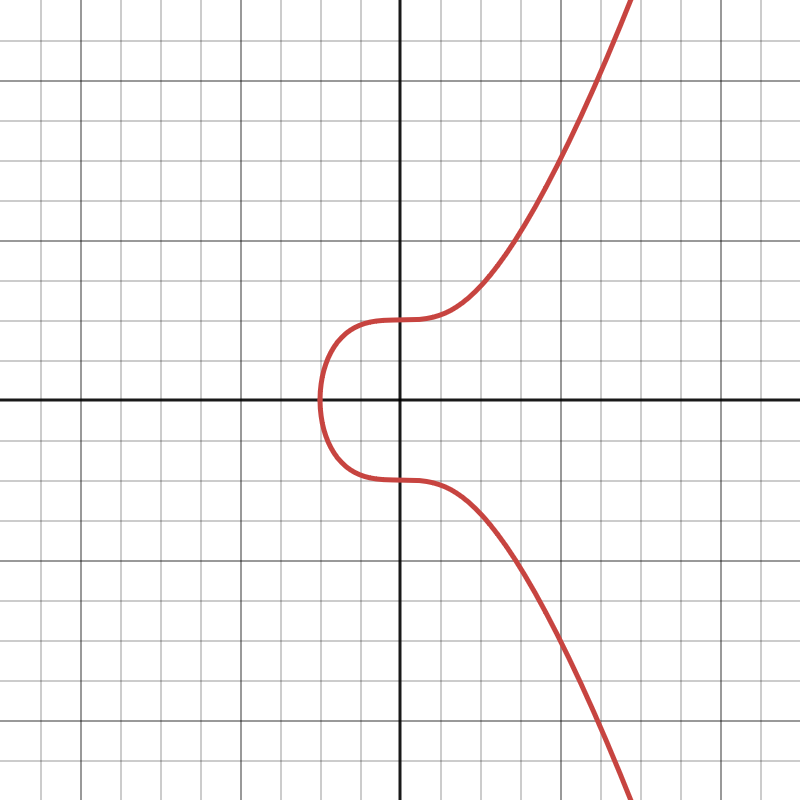
\includegraphics[width=0.2\linewidth]{images/curve-a0-b1.png}
    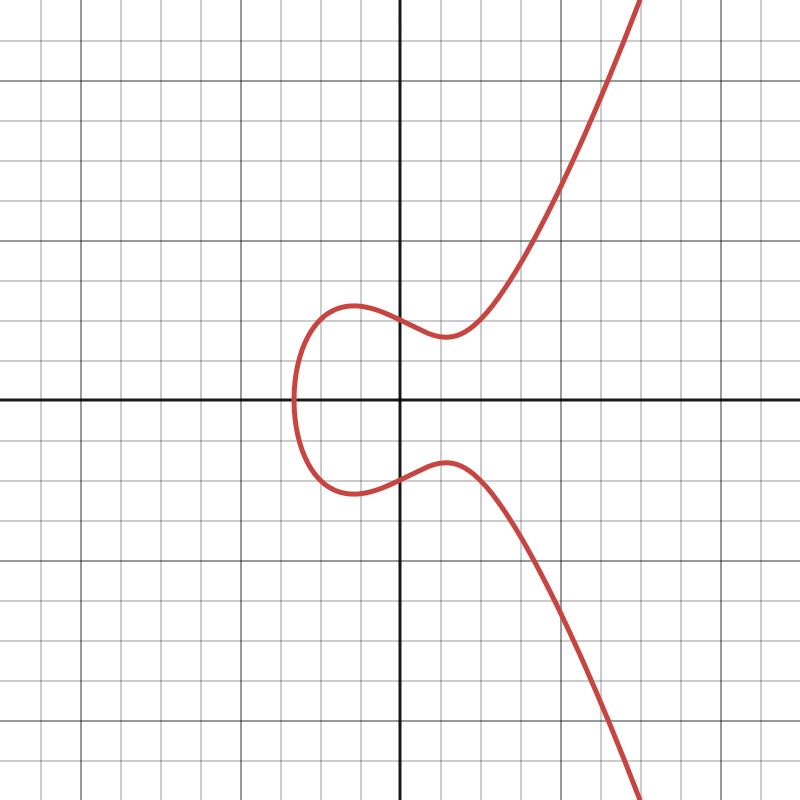
\includegraphics[width=0.2\linewidth]{images/curve-a-1-b1.png}
    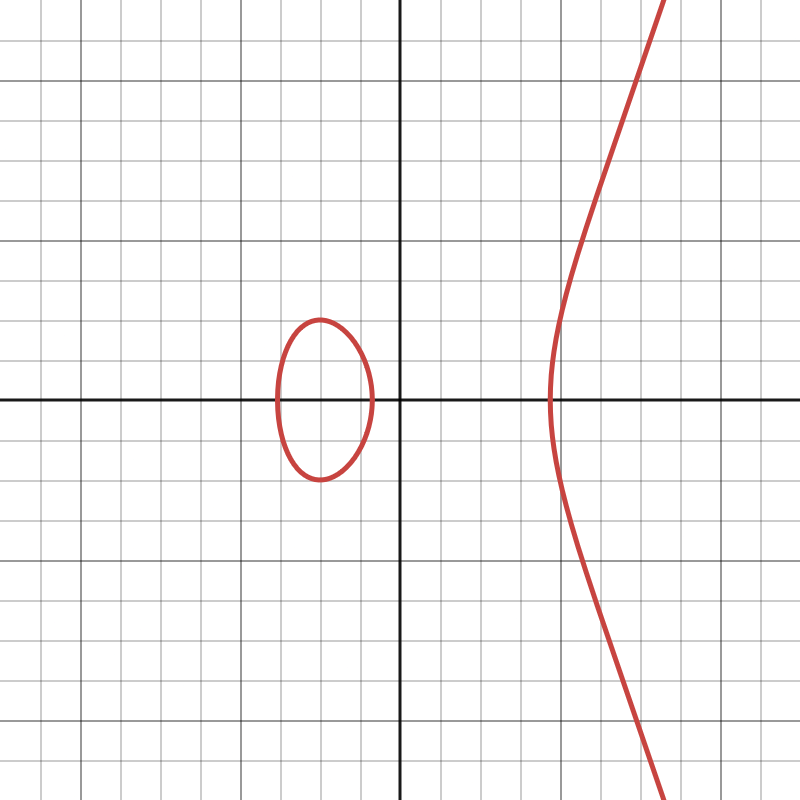
\includegraphics[width=0.2\linewidth]{images/curve-a-3-b-1.png}
    \caption{Several elliptic curves with different parameters.}
    \label{fig:curves}
\end{figure}

Some important properties of elliptic curves to consider:
\begin{enumerate}
    \item They are symmetrical across the x-axis.
    \item The "tails" of an elliptic curve are asymptotic --- they get steeper as you go further along them.
\end{enumerate}


\section{Elliptic curve point arithmetic}

The points of an elliptic curve have certain properties that enable us to form a group with a specially defined operation of addition. To understand what this means, we need to take a look at abelian groups.

\subsection{Abelian groups}

An abelian group \textit{under a certain operation} is a group for which that operation is closed, commutative and associative, and for which there exists an inverse for every element and an identity element.\cite[p. 11]{wp}

A group $G$ that acts as an abelian group under an operation addition, $+$, is written as $(G, +)$. In other words, an abelian group $(G, +)$ has the following properties for all elements $A \in G$:
\begin{enumerate}
    \item \textbf{Commutativity.} $A + B = B + A$.
    \item \textbf{Associativity.} $(A + B) + C = A + (B + C)$.
    \item \textbf{Identity element.} There exists an element $I$ such that $A + I = I + A = A$.
    \item \textbf{Inverse elements.} There exists an inverse $-A$ for every element $A$ such that $A + -A = -A + A = I$.\cite[p. 11]{guide}
\end{enumerate}

An example of an abelian group is the integers under addition $(\mathbb{Z}, +)$, with the identity element $0$. 

An example of something that is \textit{not} an abelian group is the real numbers under multiplication $(\mathbb{R}, \times)$, because $0$ has no inverse. However, the real numbers excluding $0$ is an abelian group $(\mathbb{R} \setminus \{0\}, \times)$ with identity element $1$.

\subsection{Point addition \& doubling}

The points of an elliptic curve --- the pairings $(x,y)$ that satisfy the equation of the curve --- form an abelian group under an operation which we define as addition. 

Importantly, the addition of two points $(x_1, y_1) + (x_2, y_2) \ne (x_1 + x_2, y_1 + y_2)$; point addition is \textbf{not} vector addition. Rather, the addition of points on an elliptic curve is best illustrated graphically:

\begin{figure}[h]
    \centering
    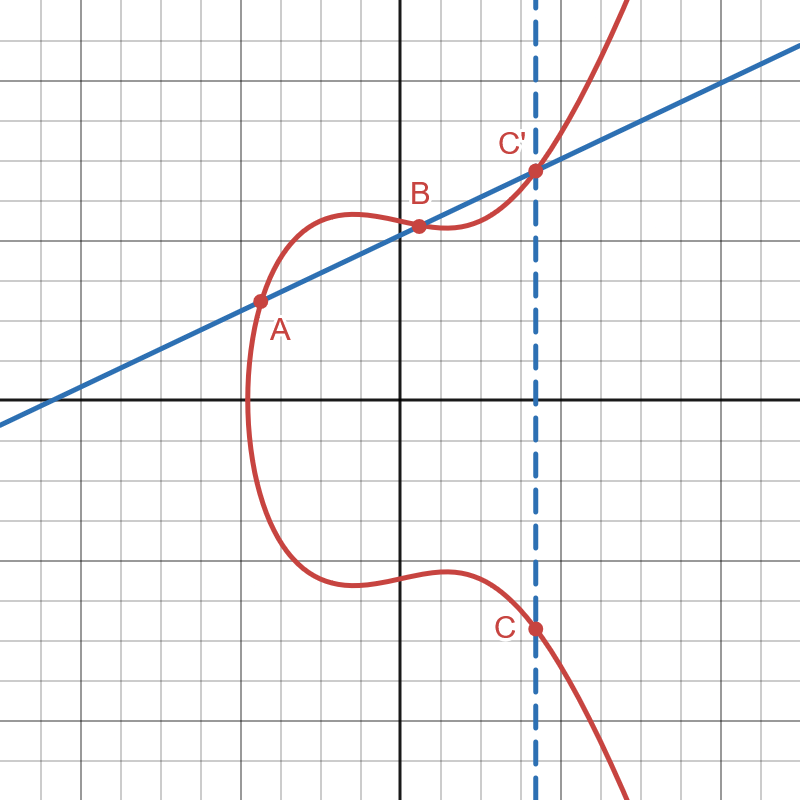
\includegraphics[width=0.3\linewidth]{images/add-add.png}
    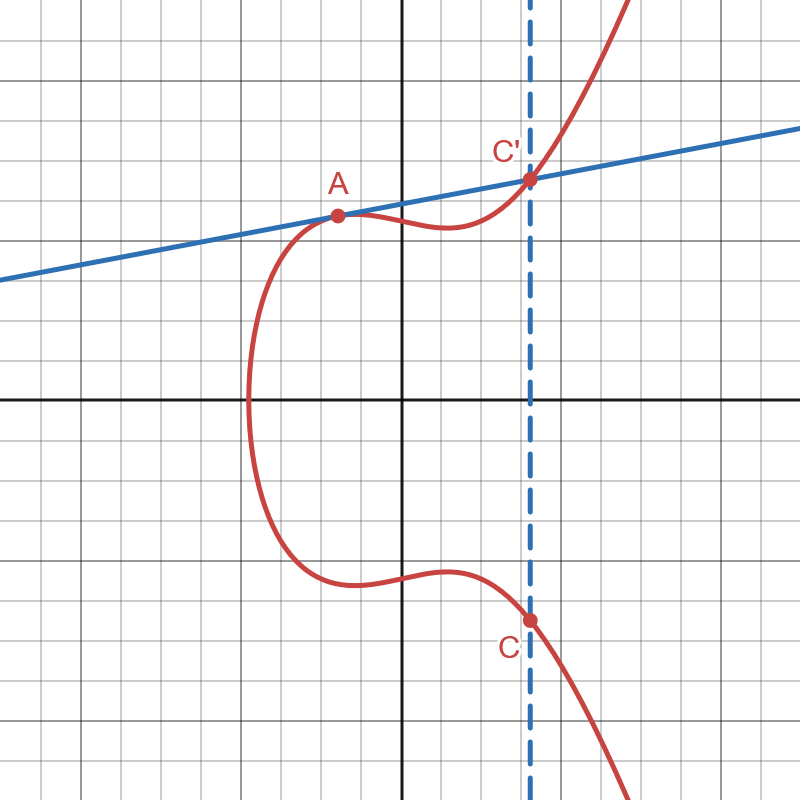
\includegraphics[width=0.3\linewidth]{images/add-double.png}
    \caption{Elliptic curve point addition and doubling..}
    \label{fig:add}
\end{figure}

To add two points $A$ and $B$: 
\begin{enumerate}
    \item Draw a line between the points $AB$.
    \item A line that intersects an elliptic curve at two points will \textit{always} intersect the curve at a third point (except for special cases, see Section \ref{poi} on the point at infinity).
    
    The second property of elliptic curves listed in Section \ref{intro} makes it intuitive that even a line that appears "too steep" will always intersect the curve eventually.
    \item Take the third point and reflect it across the x-axis to obtain point $C$.
    \item $A + B = C$
\end{enumerate}

The process is similar for adding a point to itself (point doubling), where a line cannot be drawn between two points:
\begin{enumerate}
    \item Draw a line tangential to the curve at point A.
    \item The line will intersect the curve again at another point.
    \item Take the second point and reflect it across the x-axis to obtain point $C$.
    \item $A + A = C$
\end{enumerate}

Also important to note is that every point $A(x, y)$ has an inverse $-A(x, -y)$ in order to satisfy the properties of an abelian group. This property is used when defining the point at infinity (Section \ref{poi}).

\subsection{Derivation of point addition \& doubling equations}\label{proof}

Take two points on an elliptic curve $E$ where $A(x_1, y_1) + B(x_2, y_2) = C(x_3, y_3)$ . Let the line through $A$, $B$ and $-C(x_3, -y_3)$ be $L$ such that
\begin{gather*}
    E: y^2 = x^3 + ax + b \\
    L: y = \lambda x + m \\
    \text{where } \lambda = \frac{y_2-y_1}{x_2-x_1}
\end{gather*}

The intersection of $E$ and $L$ satisfies the equation
\begin{align*}
    x^3 + ax + b = (\lambda x + m)^2 \\
    x^3 + ax + b = \lambda^2 x^2 + 2 \lambda x m + m^2 \\
    x^3 - \lambda^2 x^2 + (a - 2 \lambda m)x + b - m^2 = 0
\end{align*}

We also know this equation has roots at $x_1$, $x_2$ and $x_3$, and can be written as
\begin{align*}
    (x-x_1)(x-x_2)(x-x_3)=0 \\
    x^3 - (x_1 + x_2 + x_3)x^2 + (x_1x_2 + x_1x_3 + x_2x_3)x - x_1x_2x_3 = 0
\end{align*}

Comparing coefficients of $x^2$ in the two forms of the equation, we can see that \[\lambda^2 = x_1 + x_2 + x_3\] and therefore \[x_3 = \lambda^2 - x_1 - x_2\] which gives the equation for $x_3$. To find $y_3$, we use the fact that $\lambda$ is also equal to the gradient between $-C(x_3, -y_3)$ and $B$:
\begin{align*}
    \lambda = \frac{-y_3-y_1}{x_3-x_1} \\
    -y_3 - y_1 = \lambda(x_3-x_1) \\
    y_3 = \lambda(x_1-x_3)-y_1
\end{align*}
and we have the equation for $y_3$.\cite{proof}

Adapting these equations for point doubling $A + A = C$ is easy; as the line is no longer through two points but rather the tangent at $A$, we differentiate $E$ to find the new gradient $\lambda$:
\begin{align*}
    y^2 = x^3 + ax + b \\
    2y\frac{dy}{dx} = 3x^2 + a \\
    \frac{dy}{dx} = \frac{3x^2 + a}{2y}
\end{align*}
and so \[\lambda = \frac{3x_1^2 + a}{2y_1}\]

Also, as $x_1 = x_2$, the equation for $x_3$ becomes \[x_3 = \lambda^2-2x_1\]

The equation for $y_3$ is unchanged.

\subsection{Point at infinity}\label{poi}

When the points of an elliptic curve are used as an abelian group $(G, +)$, we have to define an identity element. We call this identity element the \textit{point at infinity}, which is written as $\infty$, $\mathcal{O}$ or $0$. This is a point that lies on the curve which we imagine to be at $(\infty, \infty)$ and that satisfies the equations
\begin{enumerate}
    \item $A + \infty = \infty + A = A$
    \item $\infty + \infty = \infty$\cite{guide}
\end{enumerate}

The point at infinity is the result of two operations:
\begin{enumerate}
    \item Adding a point to its own inverse, so $A + -A = \infty$.
    \item Doubling the point $A$ that is vertically tangential to the curve, where $2A = \infty$. This is because $A = -A$ for that point.
\end{enumerate}

\begin{figure}[h]
    \centering
    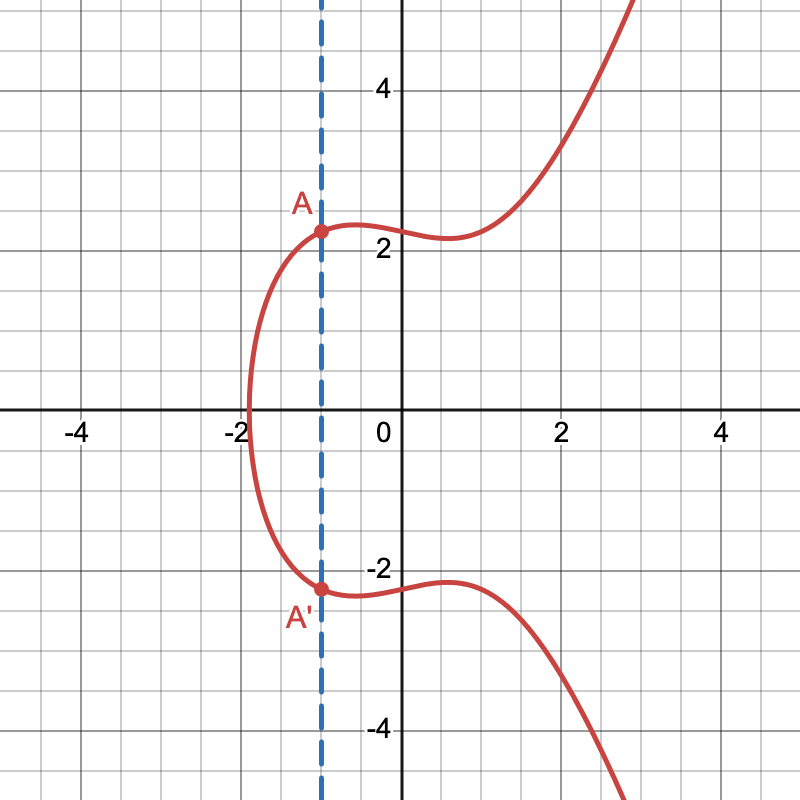
\includegraphics[width=0.3\linewidth]{images/infty-inverse.png}
    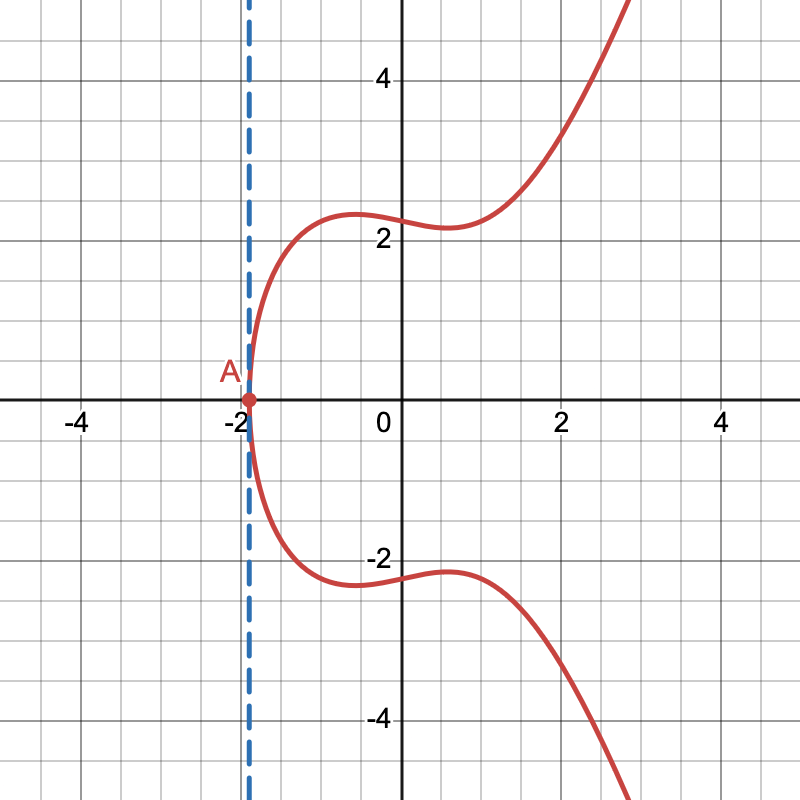
\includegraphics[width=0.3\linewidth]{images/infty-tangent.png}
    \caption{Two cases in which the point at infinity is produced.}
    \label{fig:infinity}
\end{figure}

\subsection{Point multiplication}\label{mul}

We also define an operation called point scalar multiplication. Importantly, this isn't multiplying two points by each other: rather, it is an extension of addition (and therefore not a "true" operation) where we repeatedly add a point to itself. $2A = A + A$, $3A = A + A + A$.\cite{guide}

Point scalar multiplication is important when considering the elliptic curve discrete logarithm problem (Section \ref{ecdlp}).


\section{Elliptic curves over finite fields}

Principles of discrete mathematics often emerge when discussing algorithm-related problems, and elliptic curve cryptography is no exception. Two crucial features of ECC are the elliptic curve discrete logarithm problem (ECDLP, Section \ref{ecdlp}) and the efficient one-way calculation of scalar point multiples (Section \ref{mul}). Both of these depend on the use of modular arithmetic to create finite fields.

\subsection{Finite fields}

Modular arithmetic is often called "clock face arithmetic" because of the likening of restricting calculations modulo $n$ to wrapping numbers around a clock.

% Add diagram?

Performing arithmetic modulo a number $n$ can be thought of as doing specially defined operations on a finite group --- or rather, a special subcategory of group called a field, where multiplication with certain properties is defined as well as addition.

We denote the finite field of integers modulo $n$ as $\mathbb{Z}_n$. This group has only a finite number of elements; for example, the finite field over which we do arithmetic modulo $29$ --- $\mathbb{Z}_{29}$ --- contains only the numbers $\{0, 1, \dots, 28\}$, which is where the label "finite field" comes from.

However, not every group produced by modular arithmetic is a finite field. An important axiom in the definition of a field is that in multiplication, every element except the additive identity element ($0$) has an inverse; i.e. every element $A$ has an element $-A$ for which $A \times -A = 1 \pmod{n}$. This is only true for elements which are co-prime to the modulus $n$.\cite{discrete}.

Following on from this, we can see that finite fields are only produced modulo a prime $p$, such that \textit{every} element of the set is co-prime to $p$ except $0$, and therefore has an inverse.\cite{discrete}

\subsection{Elliptic curves over finite fields}

We can define an elliptic curve $E: y^2 = x^3 + ax + b$ over a field $F$ (written as $E/F$), where the points of the elliptic curve $(x, y)$ are all such that $x, y \in F$ and $a, b \in F$ (which follows if all coordinates are in $F$ and multiplication is closed).

Elliptic curves can also be defined in this way over a finite field $\mathbb{Z}_n$, where $E: y^2 = x^2 + ax + b \pmod n$ --- see Figure \ref{fig:finite}. These curves also have a finite number of points --- the number of points, including the point at infinity, is called the \textit{order} of the curve.\cite{guide}

\begin{figure}[h]
    \centering
    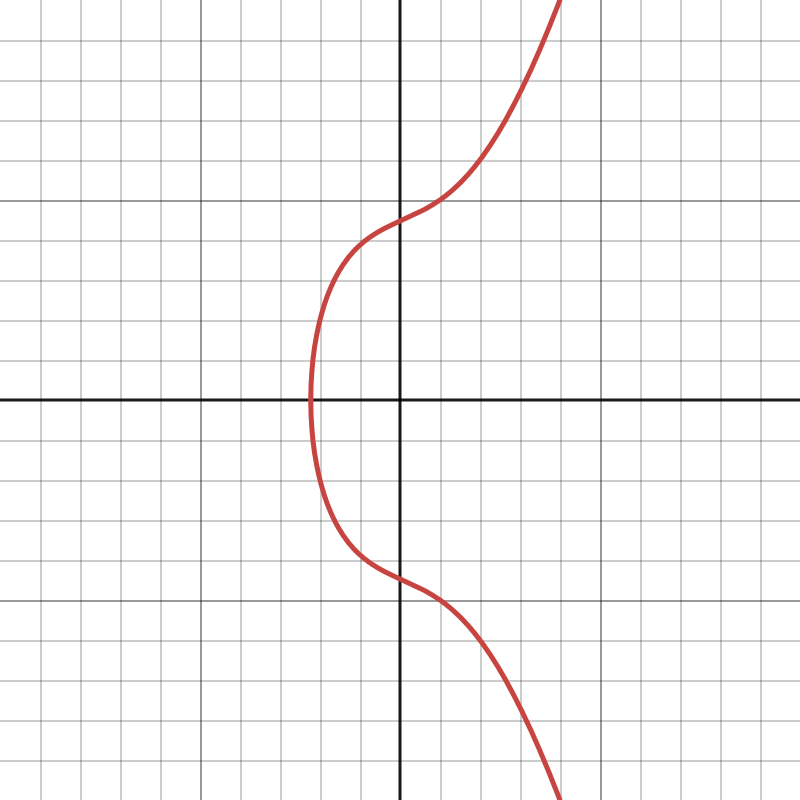
\includegraphics[width=0.3\linewidth]{images/finite-graph.png}
    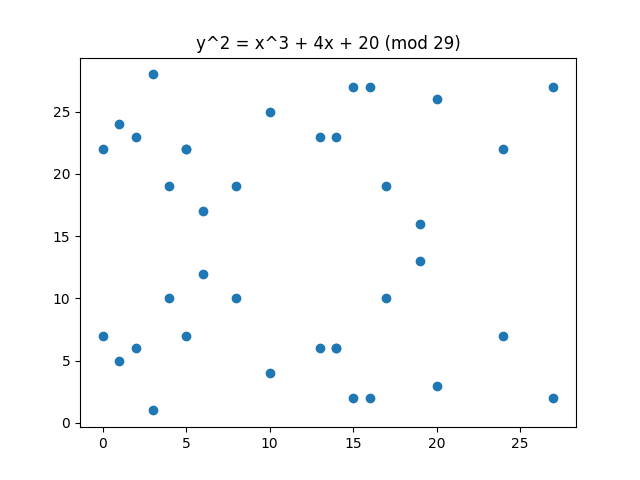
\includegraphics[width=0.4\linewidth]{images/finite-plt.png}
    \caption{$y^2=x^3+4x+20$ over $\mathbb{R}$ and $\mathbb{Z}_{29}$}
    \label{fig:finite}
\end{figure}

The equations derived in Section \ref{proof} hold for elliptic curves over finite fields as well, but division modulo $p$ must replace "regular" division over $\mathbb{R}$. This can be done using Euclid's extended algorithm for division\cite{discrete} or modular exponentiation.

Visually, these adjustments can be explained by allowing the drawn lines to wrap around the field of points until it exactly intersects another point.\cite{rareskills}

\begin{figure}[h]
    \centering
    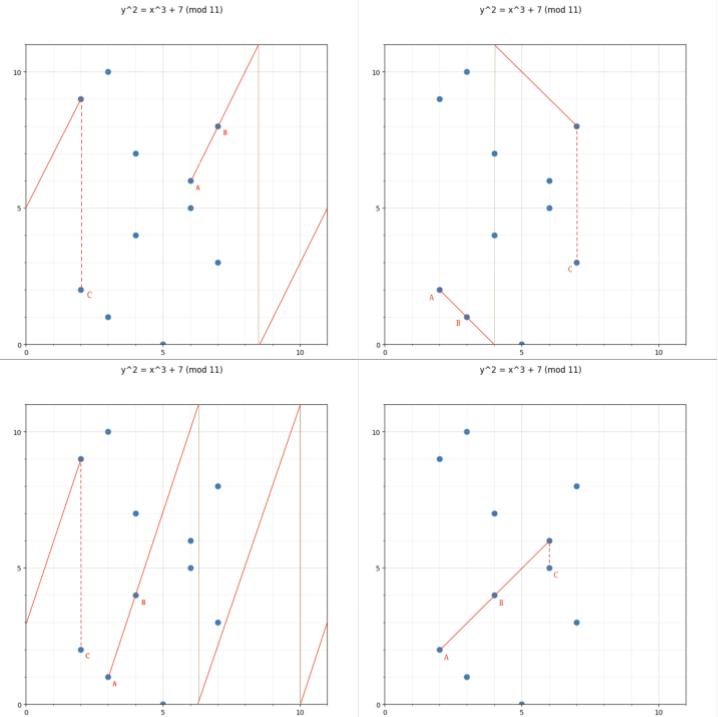
\includegraphics[width=0.5\linewidth]{images/rareskills-finite.jpg}
    \caption{Point multiplication over finite fields. Credit: RareSkills.}
\end{figure}

\subsection{Cyclical groups \& subgroups}

An interesting property of elliptic curves over finite fields is that the points of the curve will form a group that is not only abelian, but also cyclical. This means that repeated addition (point multiplication) from a generator point $G$ will produce every point on the curve once, before repeating after reaching the inverse $-G$.

Importantly, this is only true if the field is a prime finite field $\mathbb{Z}_p$. Otherwise, not every point can act as a generator, and some chosen generator points may form a "subgroup" which has a period less than the order of the curve --- therefore, not every point can be produced.\cite{practical} This is one of the reasons why the curves used in elliptic curve cryptography must be carefully chosen (see Section \ref{weak}).


\section{Public key cryptography with elliptic curves}

\subsection{The elliptic curve discrete logarithm problem (ECDLP)}\label{ecdlp}

One key property of elliptic curve point multiplication is that for certain elliptic curves, attempting to find $k$ where $kG = A$ given $G$ and $A$ is computationally difficult --- that is, it is conjectured to be hard to reverse point multiplication.\cite{practical}

This property is called the \textit{elliptic curve discrete logarithm problem} due to its similarity to the discrete logarithm problem used in cryptographic protocols like Diffie-Hellman key exchange.\cite{discrete} The elliptic curve variant is preferable for several reasons, most notably increased speed and efficiency,\cite{nist2} as well as providing more security for lower key sizes.\cite{nist}.

Several algorithms exist that speed up the computation of point multiplication, most commonly the sliding window method which decomposes large scalar multiples into several easier-to-calculate operations. However, current algorithms to reverse the calculation are not much better than the naive method (trial-and-error)\cite{guide} and have been that way for a long time. 

This gives elliptic curve cryptography a great profile to be considered for use as a trapdoor function in cryptography.\cite{nist} We will cover one protocol as an example of the use of elliptic curves in cryptography, the elliptic curve variant of Diffie-Hellman key exchange.

\subsection{Elliptic Curve Diffie-Hellman (ECDH)}

One of the most common uses of elliptic curves is in a modified Diffie-Hellman key exchange protocol, which is originally based on number theory's discrete logarithm problem. The set up is as follows:

Two clients, Alice and Bob, choose a generator points $G$ on an elliptic curve $E/\mathbb{Z}_p$ which act as their public keys. Both clients also choose their own private keys $p$ and $q$ respectively, which are random integers between $0$ and the order of the elliptic curve.

Alice calculates $p \times G$ to produce the point $A$, and sends it to Bob. Due to the elliptic curve discrete logarithm problem, any eavesdroppers cannot calculate  $p$ given $G$ and $A$. Bob similarly calculates $q \times G$ to produce $B$.

Alice then calculates $p \times B$ and Bob calculates $q \times A$ to produce the same point $P$. This is because 
\begin{align*}
    (G \times p) \times q = (G \times q) \times p \\
    = (G + G + \dots + G) + (G + G + \dots + G) \\
    = G \times (p + q)
\end{align*}
which follows from the commutative property of elliptic curve point addition.

This way, two clients can communicate over an unsecured network to derive a common secret key using the ECDLP.\cite{practical}


\section{ECC in the future of cryptography}

Despite being robust, efficient and currently in wide-scale usage, the dependence of elliptic curves in cryptography schemes is not future-proof.

\subsection{Weaknesses}\label{weak}
Programs using elliptic curve cryptography, due to the nature of the algorithms used for point multiplication, are vulnerable to side-channeling attacks.\cite{nist} These are attacks which make use of physical properties such as magnetic fluctuations, current and temperature of computers to gain insight into the workings of a program. This is known to even affect virtual machines hosted on the cloud, and the ability of hypervisors to prevent this type of "spying" is limited.\cite{cloud}

Furthermore, DUAL\_EC\_DRBG\cite{blog}

\subsection{Post-quantum cryptography}

Arguably the most notable weakness of elliptic curve cryptography is its vulnerability to quantum computers.\cite{that one really short paper} The ECDLP, much like the regular discrete logarithm problem, is solved in polynomial time by a modified version of Shor's algorithm, with only 1 million Tornelli gates.\cite{that one with gates. also correct this}

- sndl - cite... something?
- lattice-based methods
    - svp, lwe


\section{Accompanying program}

This paper was written in conjunction with a Python program, \href{https://github.com/shrub719/edu-ecc/}{Edu-ECC}, which implements the mathematics described above in an ECDH cryptography scheme with several graphical demonstrations. The program, along with documentation, is available on GitHub: \url{https://github.com/shrub719/edu-ecc/}.


\newpage
\bibliographystyle{jox}
\bibliography{bibliography}

\end{document}